\section{Durchführung}
\label{sec:Durchführung}
Der Versuch wird mit einer Messaparatur nach Abbildung \ref{fig:Messapparatur}
durchgeführt.
\begin{figure}[H]
  \centering
  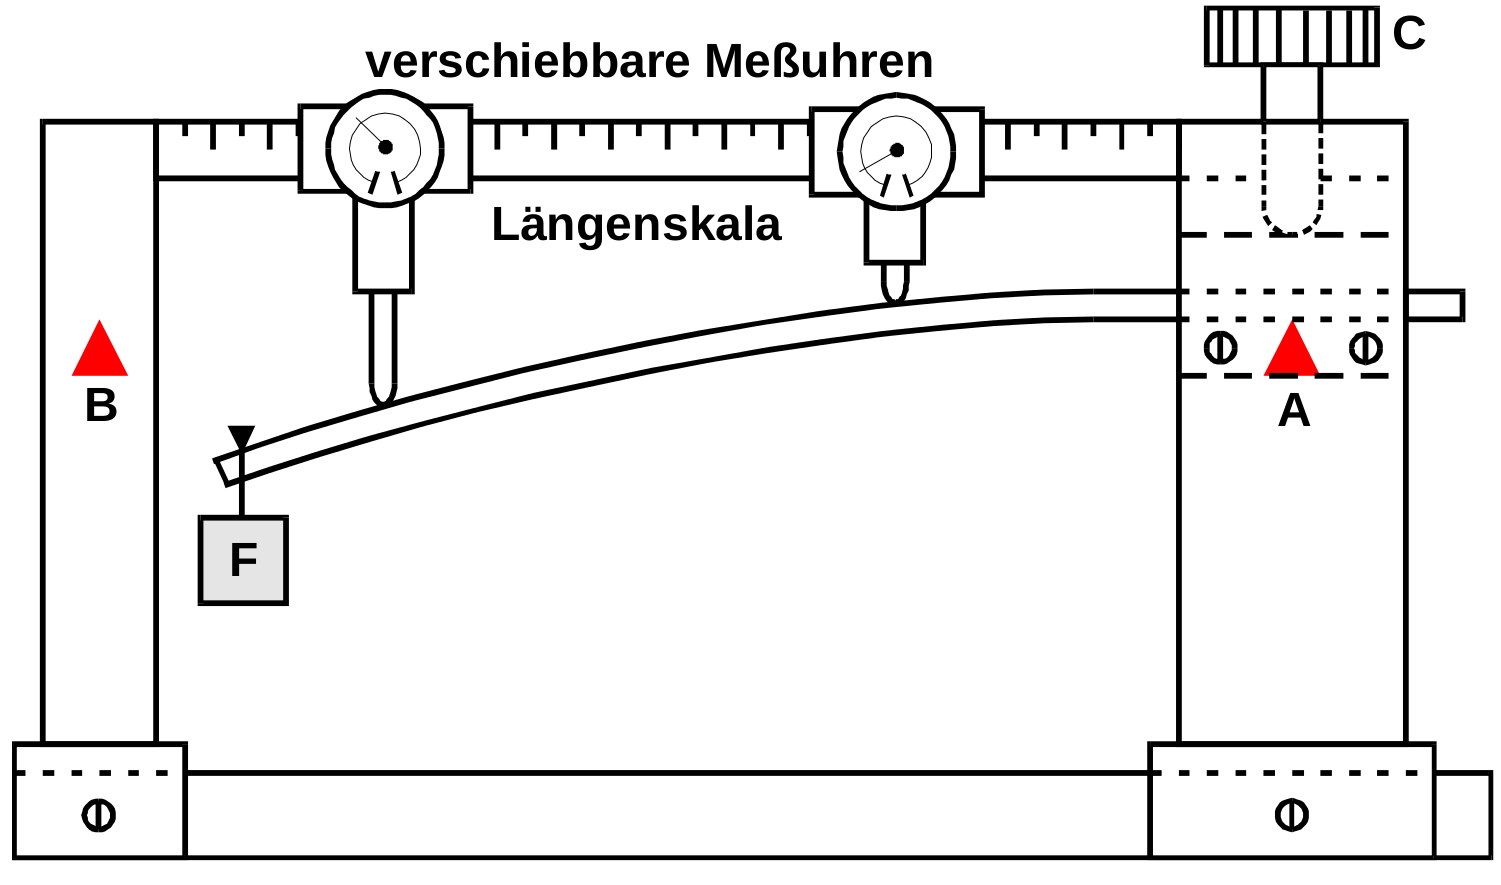
\includegraphics[width=0.5\textwidth]{Messapparatur.png}
  \caption{Darstellung einer Messapparatur zur Biegung von Stäben \cite{sample} .}
  \label{fig:Messapparatur}
\end{figure}
Die Maße des Stabes werden bestimmt sowie sein Gewicht. Mit den Messungen wird die
Dichte des Stabes und damit dessen Material bestimmt. Es wird mit den Messuhren
an verschiedenen Stellen die relative Verbiegung gemessen. Dafür wird
eine Messung mit und eine ohne Gewicht am freien Ende an jeder Messstelle
durchgeführt und die Differenz bestimmt sowie der Abstand vom Einspannpunkt notiert.
In einer zweiten Messreihe wird der Probestab auf die Auflagepunkte A und B aus
Abbildung \ref{fig:Messapparatur} gelegt. Das Gewicht wird mittig zwischen beiden
plaziert. Die relative Verbiegung wird gemessen, indem die Differenz der angezeigten
Werte bei der jeweiligen Messuhr gebildet wird. Für beide Messreihen werden
jeweils mindestens 30 Messungen gemacht. Die einseitige Messung wird für einen
 rechteckigen und einen runden Stab durchgeführt, die Messung bei beidseitiger
 Auflage nur für den rechteckigen Stab.
